%________________________________________________________________________________________
% @brief    LaTeX2e Resume for Kamil K Wojcicki
% @author   Kamil K Wojcicki
% @url   http://linux.dsplabs.com.au/?p=54
% @date     Decemebr 2007
% @info     Based on Latex Resume Template by Chris Paciorek 
%        http://www.biostat.harvard.edu/~paciorek/
%________________________________________________________________________________________
\documentclass[margin,line,a4paper]{resume}

\usepackage[utf8]{inputenc} %utf8
\usepackage[english,danish]{babel}
\usepackage[T1]{fontenc}
\usepackage{graphicx,wrapfig}
\usepackage{url}
\usepackage[colorlinks=true, a4paper=true, pdfstartview=FitV,
linkcolor=blue, citecolor=blue, urlcolor=blue]{hyperref}
\pdfcompresslevel=9


\begin{document}
\mytitle{Rian Adam}
\begin{resume}
    \vspace{0.5cm}
    \begin{wrapfigure}{R}{0.3\textwidth}
        \vspace{-1cm}
       \begin{center}
       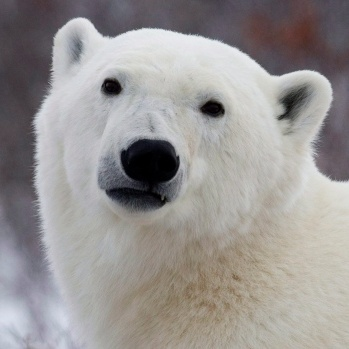
\includegraphics[width=0.3\textwidth]{foto}
       \end{center}
        \vspace{-1cm}
    \end{wrapfigure}
    


    \section{\mysidestyle{Personal\\Information}}%\vspace{2mm}
    Rian Adam \\
    899 Richardson St.Ozone Park, NY 11417 \\ 
    USA \\ 
    \textbf{Mobile} +62 123 456 789  \\
    \textbf{Email} \href{mailto:rian.adam.r@gmail.com}{rian.adam.r@gmail.com} \\
    \textbf{Sex} Male \\ 
    \textbf{Date of birth} 27/05/1994 \\ 
    \textbf{Nationality} Indonesian \\
    % \href{http://www.tjansson.dk}{www.tjansson.dk}\\    

    % I was born and raised in Copenhagen where I have liv\-ed all my life except \ldots{}
My research interest lies in applying machine learning to address real-world industrial problems. My research is driven by a strong desire to make the benefits of machine learning can be felt directly by the community. With a prior knowledge of mathematics, algorithms, and computational thinking that I gained when learning competitive programming since high school, I always try to explore the application of machine learning both theoretically and practically.

    \section{\mysidestyle{Education}} 
    
    \textbf{Masters degree in Computer Science (2016-2018)} \\
    from University of Polar Bear, Indonesia.
    \begin{itemize}
        \item {Thesis} : Fish Catching Algorithm using Fourier Transform
        \item {Grade} : 3.63 (Scale 4)
    \end{itemize}
    
     \textbf{Bachelor degree in Computer Science (2012-2016)} \\
    from University of Polar Bear, Indonesia.
    \begin{itemize}
        \item {Thesis} : How to Survive in North Pole Wihout Any Clothes
        \item {Grade} : 3.50 (Scale 4)
    \end{itemize}

\section{\mysidestyle{Job experiences}}\vspace{1mm}
\begin{description}
    
    \item[2017 May $\rightarrow$ Present] Full-time Polar Bear with full responsibility to lead our group move from one place to another place safely.
    \item[2015 October $\rightarrow$ Present] Part-time Polar Bear, with main role is catching fish for my group and survive in North pole.
 
\end{description}


\section{\mysidestyle{Publications}}

    Adam, Rian, 2017, "How to Survive in North Pole Wihout Any Clothes", Prociding of Cold Conference for Antarctic People
    
    The article was the published work of my bachelors project in 2016. 

\section{\mysidestyle{Selected Honours and Awards}}\vspace{1mm}

\begin{description}
    \item[2019] Scholarship for citizen of North Pole
    \item[2018] My latest award
    \item[2016] Second position on running competition
    \item[2015] My first award
\end{description}

% Lorem ipsum dolor sit amet, consectetur adipiscing elit, sed do eiusmod tempor incididunt ut labore et dolore magna aliqua. 

% \begin{itemize}
%     \item \emph{Review: ``Kvantespring i det 20. århundrede''}, Gamma,
%     fall, 2008.
%     \item \emph{Review: ``Insultingly stupid movie physics''}, Kvant 3,
%     2008.
%     \item \emph{Eksperiment med flydende metaller relateret til jordens
%     magnetfelt}, Gamma 145, 2007.
% \end{itemize}

\end{resume}
\end{document} 
